% IEEEtran V1.7 and later provides for these CLASSINPUT macros to allow the
% user to reprogram some IEEEtran.cls defaults if needed. These settings
% override the internal defaults of IEEEtran.cls regardless of which class
% options are used. Do not use these unless you have good reason to do so as
% they can result in nonIEEE compliant documents. User beware. ;)
%
%\newcommand{\CLASSINPUTbaselinestretch}{1.0} % baselinestretch
%\newcommand{\CLASSINPUTinnersidemargin}{1in} % inner side margin
%\newcommand{\CLASSINPUToutersidemargin}{1in} % outer side margin
%\newcommand{\CLASSINPUTtoptextmargin}{1in}   % top text margin
%\newcommand{\CLASSINPUTbottomtextmargin}{1in}% bottom text margin




%
\documentclass[10pt,journal,compsoc]{IEEEtran}
% If IEEEtran.cls has not been installed into the LaTeX system files,
% manually specify the path to it like:
% \documentclass[10pt,journal,compsoc]{../sty/IEEEtran}


% For Computer Society journals, IEEEtran defaults to the use of
% Palatino/Palladio as is done in IEEE Computer Society journals.
% To go back to Times Roman, you can use this code:
%\renewcommand{\rmdefault}{ptm}\selectfont





% Some very useful LaTeX packages include:
% (uncomment the ones you want to load)



% *** MISC UTILITY PACKAGES ***
%
%\usepackage{ifpdf}
% Heiko Oberdiek's ifpdf.sty is very useful if you need conditional
% compilation based on whether the output is pdf or dvi.
% usage:
% \ifpdf
%   % pdf code
% \else
%   % dvi code
% \fi
% The latest version of ifpdf.sty can be obtained from:
% http://www.ctan.org/pkg/ifpdf
% Also, note that IEEEtran.cls V1.7 and later provides a builtin
% \ifCLASSINFOpdf conditional that works the same way.
% When switching from latex to pdflatex and vice-versa, the compiler may
% have to be run twice to clear warning/error messages.






% *** CITATION PACKAGES ***
%
\ifCLASSOPTIONcompsoc
  % The IEEE Computer Society needs nocompress option
  % requires cite.sty v4.0 or later (November 2003)
  \usepackage[nocompress]{cite}
\else
  % normal IEEE
  \usepackage{cite}
\fi
% cite.sty was written by Donald Arseneau
% V1.6 and later of IEEEtran pre-defines the format of the cite.sty package
% \cite{} output to follow that of the IEEE. Loading the cite package will
% result in citation numbers being automatically sorted and properly
% "compressed/ranged". e.g., [1], [9], [2], [7], [5], [6] without using
% cite.sty will become [1], [2], [5]--[7], [9] using cite.sty. cite.sty's
% \cite will automatically add leading space, if needed. Use cite.sty's
% noadjust option (cite.sty V3.8 and later) if you want to turn this off
% such as if a citation ever needs to be enclosed in parenthesis.
% cite.sty is already installed on most LaTeX systems. Be sure and use
% version 5.0 (2009-03-20) and later if using hyperref.sty.
% The latest version can be obtained at:
% http://www.ctan.org/pkg/cite
% The documentation is contained in the cite.sty file itself.
%
% Note that some packages require special options to format as the Computer
% Society requires. In particular, Computer Society  papers do not use
% compressed citation ranges as is done in typical IEEE papers
% (e.g., [1]-[4]). Instead, they list every citation separately in order
% (e.g., [1], [2], [3], [4]). To get the latter we need to load the cite
% package with the nocompress option which is supported by cite.sty v4.0
% and later.





% *** GRAPHICS RELATED PACKAGES ***
%
\ifCLASSINFOpdf
  \usepackage[pdftex]{graphicx}
  % declare the path(s) where your graphic files are
  % \graphicspath{{../pdf/}{../jpeg/}}
  % and their extensions so you won't have to specify these with
  % every instance of \includegraphics
  \DeclareGraphicsExtensions{.pdf,.jpeg,.png}
\else
  % or other class option (dvipsone, dvipdf, if not using dvips). graphicx
  % will default to the driver specified in the system graphics.cfg if no
  % driver is specified.
  % \usepackage[dvips]{graphicx}
  % declare the path(s) where your graphic files are
  % \graphicspath{{../eps/}}
  % and their extensions so you won't have to specify these with
  % every instance of \includegraphics
  % \DeclareGraphicsExtensions{.eps}
\fi
% graphicx was written by David Carlisle and Sebastian Rahtz. It is
% required if you want graphics, photos, etc. graphicx.sty is already
% installed on most LaTeX systems. The latest version and documentation
% can be obtained at:
% http://www.ctan.org/pkg/graphicx
% Another good source of documentation is "Using Imported Graphics in
% LaTeX2e" by Keith Reckdahl which can be found at:
% http://www.ctan.org/pkg/epslatex
%
% latex, and pdflatex in dvi mode, support graphics in encapsulated
% postscript (.eps) format. pdflatex in pdf mode supports graphics
% in .pdf, .jpeg, .png and .mps (metapost) formats. Users should ensure
% that all non-photo figures use a vector format (.eps, .pdf, .mps) and
% not a bitmapped formats (.jpeg, .png). The IEEE frowns on bitmapped formats
% which can result in "jaggedy"/blurry rendering of lines and letters as
% well as large increases in file sizes.
%
% You can find documentation about the pdfTeX application at:
% http://www.tug.org/applications/pdftex





% *** MATH PACKAGES ***
%
\usepackage{amsmath, amsthm, amsfonts, amsbsy, amssymb}
\usepackage{mathtools}
\usepackage{float}
% A popular package from the American Mathematical Society that provides
% many useful and powerful commands for dealing with mathematics.
%
% Note that the amsmath package sets \interdisplaylinepenalty to 10000
% thus preventing page breaks from occurring within multiline equations. Use:
%\interdisplaylinepenalty=2500
% after loading amsmath to restore such page breaks as IEEEtran.cls normally
% does. amsmath.sty is already installed on most LaTeX systems. The latest
% version and documentation can be obtained at:
% http://www.ctan.org/pkg/amsmath





% *** SPECIALIZED LIST PACKAGES ***
%\usepackage{acronym}
% acronym.sty was written by Tobias Oetiker. This package provides tools for
% managing documents with large numbers of acronyms. (You don't *have* to
% use this package - unless you have a lot of acronyms, you may feel that
% such package management of them is bit of an overkill.)
% Do note that the acronym environment (which lists acronyms) will have a
% problem when used under IEEEtran.cls because acronym.sty relies on the
% description list environment - which IEEEtran.cls has customized for
% producing IEEE style lists. A workaround is to declared the longest
% label width via the IEEEtran.cls \IEEEiedlistdecl global control:
%
% \renewcommand{\IEEEiedlistdecl}{\IEEEsetlabelwidth{SONET}}
% \begin{acronym}
%
% \end{acronym}
% \renewcommand{\IEEEiedlistdecl}{\relax}% remember to reset \IEEEiedlistdecl
%
% instead of using the acronym environment's optional argument.
% The latest version and documentation can be obtained at:
% http://www.ctan.org/pkg/acronym


%\usepackage{algorithmic}
% algorithmic.sty was written by Peter Williams and Rogerio Brito.
% This package provides an algorithmic environment fo describing algorithms.
% You can use the algorithmic environment in-text or within a figure
% environment to provide for a floating algorithm. Do NOT use the algorithm
% floating environment provided by algorithm.sty (by the same authors) or
% algorithm2e.sty (by Christophe Fiorio) as the IEEE does not use dedicated
% algorithm float types and packages that provide these will not provide
% correct IEEE style captions. The latest version and documentation of
% algorithmic.sty can be obtained at:
% http://www.ctan.org/pkg/algorithms
% Also of interest may be the (relatively newer and more customizable)
% algorithmicx.sty package by Szasz Janos:
% http://www.ctan.org/pkg/algorithmicx




% *** ALIGNMENT PACKAGES ***
%
%\usepackage{array}
% Frank Mittelbach's and David Carlisle's array.sty patches and improves
% the standard LaTeX2e array and tabular environments to provide better
% appearance and additional user controls. As the default LaTeX2e table
% generation code is lacking to the point of almost being broken with
% respect to the quality of the end results, all users are strongly
% advised to use an enhanced (at the very least that provided by array.sty)
% set of table tools. array.sty is already installed on most systems. The
% latest version and documentation can be obtained at:
% http://www.ctan.org/pkg/array


%\usepackage{mdwmath}
%\usepackage{mdwtab}
% Also highly recommended is Mark Wooding's extremely powerful MDW tools,
% especially mdwmath.sty and mdwtab.sty which are used to format equations
% and tables, respectively. The MDWtools set is already installed on most
% LaTeX systems. The lastest version and documentation is available at:
% http://www.ctan.org/pkg/mdwtools


% IEEEtran contains the IEEEeqnarray family of commands that can be used to
% generate multiline equations as well as matrices, tables, etc., of high
% quality.


%\usepackage{eqparbox}
% Also of notable interest is Scott Pakin's eqparbox package for creating
% (automatically sized) equal width boxes - aka "natural width parboxes".
% Available at:
% http://www.ctan.org/pkg/eqparbox




% *** SUBFIGURE PACKAGES ***
%\ifCLASSOPTIONcompsoc
%  \usepackage[caption=false,font=footnotesize,labelfont=sf,textfont=sf]{subfig}
%\else
%  \usepackage[caption=false,font=footnotesize]{subfig}
%\fi
% subfig.sty, written by Steven Douglas Cochran, is the modern replacement
% for subfigure.sty, the latter of which is no longer maintained and is
% incompatible with some LaTeX packages including fixltx2e. However,
% subfig.sty requires and automatically loads Axel Sommerfeldt's caption.sty
% which will override IEEEtran.cls' handling of captions and this will result
% in non-IEEE style figure/table captions. To prevent this problem, be sure
% and invoke subfig.sty's "caption=false" package option (available since
% subfig.sty version 1.3, 2005/06/28) as this is will preserve IEEEtran.cls
% handling of captions.
% Note that the Computer Society format requires a sans serif font rather
% than the serif font used in traditional IEEE formatting and thus the need
% to invoke different subfig.sty package options depending on whether
% compsoc mode has been enabled.
%
% The latest version and documentation of subfig.sty can be obtained at:
% http://www.ctan.org/pkg/subfig




% *** FLOAT PACKAGES ***
%
%\usepackage{fixltx2e}
% fixltx2e, the successor to the earlier fix2col.sty, was written by
% Frank Mittelbach and David Carlisle. This package corrects a few problems
% in the LaTeX2e kernel, the most notable of which is that in current
% LaTeX2e releases, the ordering of single and double column floats is not
% guaranteed to be preserved. Thus, an unpatched LaTeX2e can allow a
% single column figure to be placed prior to an earlier double column
% figure.
% Be aware that LaTeX2e kernels dated 2015 and later have fixltx2e.sty's
% corrections already built into the system in which case a warning will
% be issued if an attempt is made to load fixltx2e.sty as it is no longer
% needed.
% The latest version and documentation can be found at:
% http://www.ctan.org/pkg/fixltx2e


%\usepackage{stfloats}
% stfloats.sty was written by Sigitas Tolusis. This package gives LaTeX2e
% the ability to do double column floats at the bottom of the page as well
% as the top. (e.g., "\begin{figure*}[!b]" is not normally possible in
% LaTeX2e). It also provides a command:
%\fnbelowfloat
% to enable the placement of footnotes below bottom floats (the standard
% LaTeX2e kernel puts them above bottom floats). This is an invasive package
% which rewrites many portions of the LaTeX2e float routines. It may not work
% with other packages that modify the LaTeX2e float routines. The latest
% version and documentation can be obtained at:
% http://www.ctan.org/pkg/stfloats
% Do not use the stfloats baselinefloat ability as the IEEE does not allow
% \baselineskip to stretch. Authors submitting work to the IEEE should note
% that the IEEE rarely uses double column equations and that authors should try
% to avoid such use. Do not be tempted to use the cuted.sty or midfloat.sty
% packages (also by Sigitas Tolusis) as the IEEE does not format its papers in
% such ways.
% Do not attempt to use stfloats with fixltx2e as they are incompatible.
% Instead, use Morten Hogholm'a dblfloatfix which combines the features
% of both fixltx2e and stfloats:
%
% \usepackage{dblfloatfix}
% The latest version can be found at:
% http://www.ctan.org/pkg/dblfloatfix


%\ifCLASSOPTIONcaptionsoff
%  \usepackage[nomarkers]{endfloat}
% \let\MYoriglatexcaption\caption
% \renewcommand{\caption}[2][\relax]{\MYoriglatexcaption[#2]{#2}}
%\fi
% endfloat.sty was written by James Darrell McCauley, Jeff Goldberg and
% Axel Sommerfeldt. This package may be useful when used in conjunction with
% IEEEtran.cls'  captionsoff option. Some IEEE journals/societies require that
% submissions have lists of figures/tables at the end of the paper and that
% figures/tables without any captions are placed on a page by themselves at
% the end of the document. If needed, the draftcls IEEEtran class option or
% \CLASSINPUTbaselinestretch interface can be used to increase the line
% spacing as well. Be sure and use the nomarkers option of endfloat to
% prevent endfloat from "marking" where the figures would have been placed
% in the text. The two hack lines of code above are a slight modification of
% that suggested by in the endfloat docs (section 8.4.1) to ensure that
% the full captions always appear in the list of figures/tables - even if
% the user used the short optional argument of \caption[]{}.
% IEEE papers do not typically make use of \caption[]'s optional argument,
% so this should not be an issue. A similar trick can be used to disable
% captions of packages such as subfig.sty that lack options to turn off
% the subcaptions:
% For subfig.sty:
% \let\MYorigsubfloat\subfloat
% \renewcommand{\subfloat}[2][\relax]{\MYorigsubfloat[]{#2}}
% However, the above trick will not work if both optional arguments of
% the \subfloat command are used. Furthermore, there needs to be a
% description of each subfigure *somewhere* and endfloat does not add
% subfigure captions to its list of figures. Thus, the best approach is to
% avoid the use of subfigure captions (many IEEE journals avoid them anyway)
% and instead reference/explain all the subfigures within the main caption.
% The latest version of endfloat.sty and its documentation can obtained at:
% http://www.ctan.org/pkg/endfloat
%
% The IEEEtran \ifCLASSOPTIONcaptionsoff conditional can also be used
% later in the document, say, to conditionally put the References on a
% page by themselves.



% *** PDF, URL AND HYPERLINK PACKAGES ***
%
\usepackage{url}
% url.sty was written by Donald Arseneau. It provides better support for
% handling and breaking URLs. url.sty is already installed on most LaTeX
% systems. The latest version and documentation can be obtained at:
% http://www.ctan.org/pkg/url
% Basically, \url{my_url_here}.


% NOTE: PDF thumbnail features are not required in IEEE papers
%       and their use requires extra complexity and work.
%\ifCLASSINFOpdf
%  \usepackage[pdftex]{thumbpdf}
%\else
%  \usepackage[dvips]{thumbpdf}
%\fi
% thumbpdf.sty and its companion Perl utility were written by Heiko Oberdiek.
% It allows the user a way to produce PDF documents that contain fancy
% thumbnail images of each of the pages (which tools like acrobat reader can
% utilize). This is possible even when using dvi->ps->pdf workflow if the
% correct thumbpdf driver options are used. thumbpdf.sty incorporates the
% file containing the PDF thumbnail information (filename.tpm is used with
% dvips, filename.tpt is used with pdftex, where filename is the base name of
% your tex document) into the final ps or pdf output document. An external
% utility, the thumbpdf *Perl script* is needed to make these .tpm or .tpt
% thumbnail files from a .ps or .pdf version of the document (which obviously
% does not yet contain pdf thumbnails). Thus, one does a:
%
% thumbpdf filename.pdf
%
% to make a filename.tpt, and:
%
% thumbpdf --mode dvips filename.ps
%
% to make a filename.tpm which will then be loaded into the document by
% thumbpdf.sty the NEXT time the document is compiled (by pdflatex or
% latex->dvips->ps2pdf). Users must be careful to regenerate the .tpt and/or
% .tpm files if the main document changes and then to recompile the
% document to incorporate the revised thumbnails to ensure that thumbnails
% match the actual pages. It is easy to forget to do this!
%
% Unix systems come with a Perl interpreter. However, MS Windows users
% will usually have to install a Perl interpreter so that the thumbpdf
% script can be run. The Ghostscript PS/PDF interpreter is also required.
% See the thumbpdf docs for details. The latest version and documentation
% can be obtained at.
% http://www.ctan.org/pkg/thumbpdf


% NOTE: PDF hyperlink and bookmark features are not required in IEEE
%       papers and their use requires extra complexity and work.
\newcommand\MYhyperrefoptions{bookmarks=true,bookmarksnumbered=true,
pdfpagemode={UseOutlines},plainpages=false,pdfpagelabels=true,
colorlinks=true,linkcolor={black},citecolor={black},urlcolor={black},
pdftitle={Automatic Product Categorization for Anonymous Marketplaces},
pdfsubject={Machine Learning},
pdfauthor={Graczyk,Kinningham},
pdfkeywords={marketplaces,machine learning} }
%\ifCLASSINFOpdf
%\usepackage[\MYhyperrefoptions,pdftex]{hyperref}
%\else
%\usepackage[\MYhyperrefoptions,breaklinks=true,dvips]{hyperref}
%\usepackage{breakurl}
%\fi
% One significant drawback of using hyperref under DVI output is that the
% LaTeX compiler cannot break URLs across lines or pages as can be done
% under pdfLaTeX's PDF output via the hyperref pdftex driver. This is
% probably the single most important capability distinction between the
% DVI and PDF output. Perhaps surprisingly, all the other PDF features
% (PDF bookmarks, thumbnails, etc.) can be preserved in
% .tex->.dvi->.ps->.pdf workflow if the respective packages/scripts are
% loaded/invoked with the correct driver options (dvips, etc.).
% As most IEEE papers use URLs sparingly (mainly in the references), this
% may not be as big an issue as with other publications.
%
% That said, Vilar Camara Neto created his breakurl.sty package which
% permits hyperref to easily break URLs even in dvi mode.
% Note that breakurl, unlike most other packages, must be loaded
% AFTER hyperref. The latest version of breakurl and its documentation can
% be obtained at:
% http://www.ctan.org/pkg/breakurl
% breakurl.sty is not for use under pdflatex pdf mode.
%
% The advanced features offer by hyperref.sty are not required for IEEE
% submission, so users should weigh these features against the added
% complexity of use.
% The package options above demonstrate how to enable PDF bookmarks
% (a type of table of contents viewable in Acrobat Reader) as well as
% PDF document information (title, subject, author and keywords) that is
% viewable in Acrobat reader's Document_Properties menu. PDF document
% information is also used extensively to automate the cataloging of PDF
% documents. The above set of options ensures that hyperlinks will not be
% colored in the text and thus will not be visible in the printed page,
% but will be active on "mouse over". USING COLORS OR OTHER HIGHLIGHTING
% OF HYPERLINKS CAN RESULT IN DOCUMENT REJECTION BY THE IEEE, especially if
% these appear on the "printed" page. IF IN DOUBT, ASK THE RELEVANT
% SUBMISSION EDITOR. You may need to add the option hypertexnames=false if
% you used duplicate equation numbers, etc., but this should not be needed
% in normal IEEE work.
% The latest version of hyperref and its documentation can be obtained at:
% http://www.ctan.org/pkg/hyperref





% *** Do not adjust lengths that control margins, column widths, etc. ***
% *** Do not use packages that alter fonts (such as pslatex).         ***
% There should be no need to do such things with IEEEtran.cls V1.6 and later.
% (Unless specifically asked to do so by the journal or conference you plan
% to submit to, of course. )


% correct bad hyphenation here
\hyphenation{op-tical net-works semi-conduc-tor}

% Macro definitions
\newcommand{\RR}{\mathbb{R}}
\newcommand{\partialof}[2]{\frac{\partial #2}{\partial #1}}
\newcommand{\norm}[1]{\left\lVert#1\right\rVert}
\newcommand{\iu}{{i\mkern1mu}}
\newcommand{\argmin}{\operatornamewithlimits{argmin}\,}
\newcommand{\argmax}{\operatornamewithlimits{argmax}\,}
\newcommand{\Expect}{{\rm I\kern-.3em E}}
\newcommand*\diff{\mathop{}\!\mathrm{d}}


\begin{document}
%
% paper title
% Titles are generally capitalized except for words such as a, an, and, as,
% at, but, by, for, in, nor, of, on, or, the, to and up, which are usually
% not capitalized unless they are the first or last word of the title.
% Linebreaks \\ can be used within to get better formatting as desired.
% Do not put math or special symbols in the title.
\title{Automatic Product Categorization for Anonymous Marketplaces}
%
%
% author names
% note positions of commas and nonbreaking spaces ( ~ ) LaTeX will not break
% a structure at a ~ so this keeps an author's name from being broken across
% two lines.
\author{Michael~Graczyk, Kevin~Kinningham}

% The paper headers
\markboth{CS229 Machine Learning Final Project}%
{Graczyk,Kinningham: Automatic Product Categorization for Anonymous Marketplaces}
% The only time the second header will appear is for the odd numbered pages
% after the title page when using the twoside option.


% for Computer Society papers, we must declare the abstract and index terms
% PRIOR to the title within the \IEEEtitleabstractindextext IEEEtran
% command as these need to go into the title area created by \maketitle.
% As a general rule, do not put math, special symbols or citations
% in the abstract or keywords.
\IEEEtitleabstractindextext{%
\begin{abstract}
In this paper, we present a machine learning algorithm to classify product listings posted to
anonymous marketplaces.
We classify these listings according to the type of product being sold.
The categories are derived from the 12 product categories on a popular anonymous marketplace, Agora.
Our algorithm is a combination of TF-IDF for feature extraction, PCA for feature selection,
and SVM for classification.
We compare our algorithm to simpler models, including multinomial-event naive bayes and a baseline
algorithm that uses simple string pattern matching.  We achieve an accuracy of 79\% on a withheld
test set compared to an accuracy of 62\% our baseline model.
\end{abstract}
}

% make the title area
\maketitle


% To allow for easy dual compilation without having to reenter the
% abstract/keywords data, the \IEEEtitleabstractindextext text will
% not be used in maketitle, but will appear (i.e., to be "transported")
% here as \IEEEdisplaynontitleabstractindextext when compsoc mode
% is not selected <OR> if conference mode is selected - because compsoc
% conference papers position the abstract like regular (non-compsoc)
% papers do!
\IEEEdisplaynontitleabstractindextext
% \IEEEdisplaynontitleabstractindextext has no effect when using
% compsoc under a non-conference mode.


% For peerreview papers, this IEEEtran command inserts a page break and
% creates the second title. It will be ignored for other modes.
\IEEEpeerreviewmaketitle


\section{Introduction}\label{sec:introduction}
Anonymous marketplaces are a rapidly growing segment of online illegal drug
sales. Figures \ref{agora} and \ref{product_time} show the mainstream user
interface and product listing growth of one such site.
However, due to their clandestine nature, it can be difficult to extract information about product listings without manual intervention.
Law enforcement officials and interested researchers must have an expert manually tag each listing or rely on error prone ad-hoc methods of catagorizing product listings.

To improve this process, we developed a machine learning algorithm that can
automatically categorize listings with high accuracy. The input to our algorithm
is the listing text, including it's title and description. We then use TF-IDF to
extract features followed by PCA to select features from the text.  Finally, we
use a SVM to classifiy the features and output a product category.

All data processing and machine learning was executed using tools and algorithms
in scikit-learn \cite{scikit-learn}. Plots were generated using matplotlib
\cite{matplotlib}.
\begin{figure}[htbp]
    \begin{minipage}[t]{0.45\linewidth}
        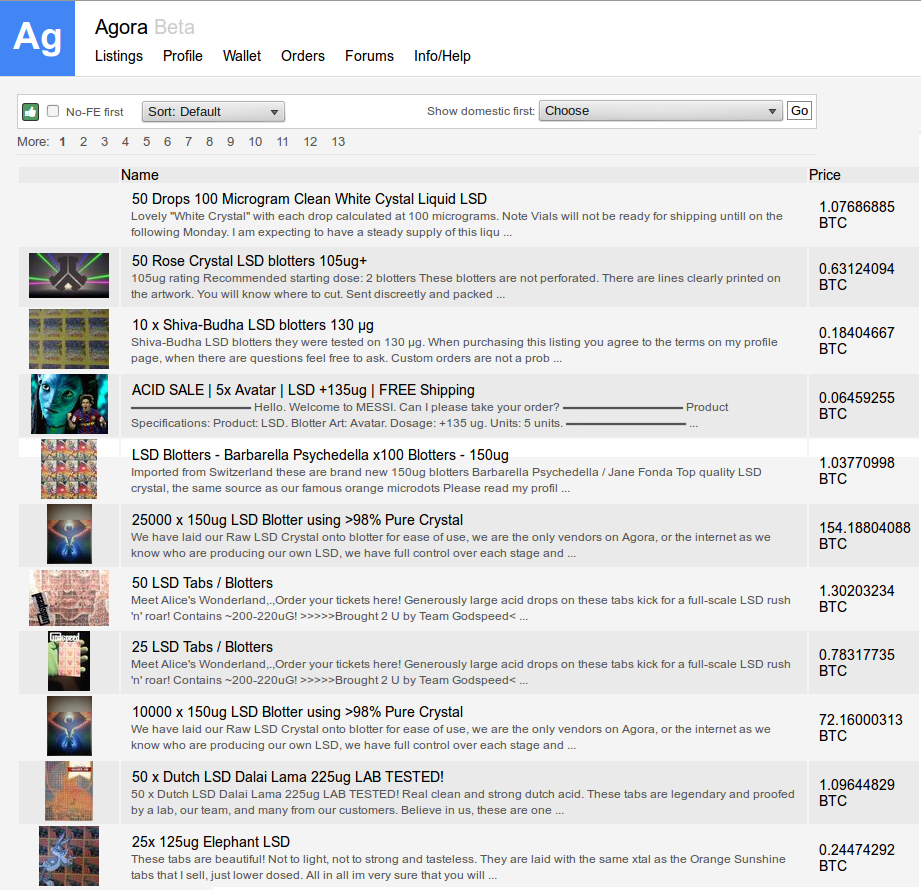
\includegraphics[width=\linewidth]{agora}
        \caption{Agora Marketplace on January 2015}
        \label{agora}
    \end{minipage}
    \hfill
    \begin{minipage}[t]{0.45\linewidth}
        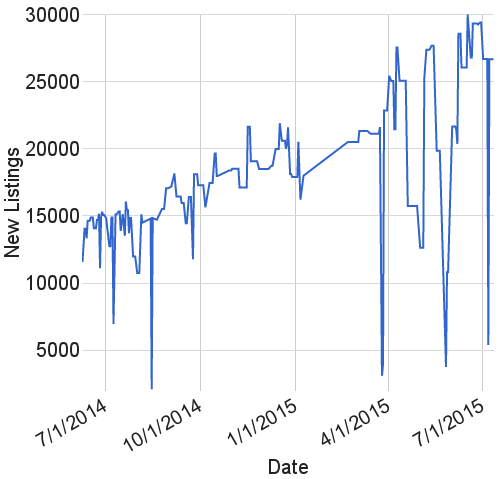
\includegraphics[width=\linewidth]{plots/new_listings_graph}
        \caption{New Product Listings Over Time}
        \label{product_time}
    \end{minipage}
\end{figure}


\section{Related Work}
There have been several attempts to analyze anonymous marketplaces\cite{gwern-silkroad}\cite{christin-silkroad}.
In \cite{christin-silkroad}, the author crawled The Silk Road for eight months, analyzing product listings and the overall distribution of product listings.
However, they relied on vendor supplied categorizations, which do not exist for all marketplaces.
Additionally, some vendors purposely misclassify their product to appear higher in marketplace search results.
Correcting for these problems requires manual labeling of at least a large fraction of the data (as has been used in analysis on other marketplaces, such as RAMP).

Most of the machine learning techniques we used are well documented in the literature as effective building blocks for document classification systems.
We extract word features from each listing using Term Frequency-Inverse Document Frequency (TF-IDF),
which has proven effective in document categorization. \cite[p. 118]{manning}.
Using SVD for dimensionality reduction is a common technique for reducing the size of the feature space for document classification\cite{sun2004supervised}.

% You should find existing papers, group them into categories based on their approaches, and talk
% about them: Discuss strengths and weaknesses. In your opinion, which approaches were clever/good?
% What is the state-of-the-art? Do most people perform the task by hand? You should aim to have at
% least 5 references in the related work. Include previous attempts by others at your problem,
% previous technical methods, or previous learning algorithms. Google Scholar is very useful for this:
% https://scholar.google.com/ (you can click “cite” and it generates MLA, APA, BibTeX, etc.)


\section{Dataset and Features}
We used an anonymous marketplace product listing dataset created by the researcher known as
Gwern\cite{gwern-darknet}.
This dataset was created by crawling several marketplaces daily, from June 6th, 2014 to July 7th, 2015.
For each product listing, we extracted the posting text, including name and description.
The resulting dataset was then cleaned to remove parse errors and duplicate listings.
We then tokenized the cleaned listings by extracting all words and numbers seperated by spaces or
symbols.
The final dataset had about 84,000 unique product listings and was used as input to feature extraction.

\begin{table}[!ht]
    \begin{center}
        \begin{tabular}{| l | p{0.8\linewidth} |}
        \hline
        Crawl Date & 2014-06-28 \\
        \hline
        Category & MDMA \\
        \hline
        Title & 28 Grams of Interways Crystal Clear Molly \\
        \hline
        Price & 1.37853692 BTC \\
        \hline
        Description & This is 28 grams of Interways crystal clear molly.
        It will be both rocky and sandy as thats how I received it.
        I am pre packaging these up accordingly and only cr... \\
        \hline
        \end{tabular}
    \end{center}
    \caption{Example product listing on Agora}
\end{table}

To convert the text to features, we used Term Frequecy-Inverse Document Frequence (TF-IDF).
TF-IDF converts each token in the listing to a token weight based on how important that token is to the listing, normalized by the number of times the token appears in the whole corpus.
This normalization helps to reduce the impact of common token in the corpus.
Finally, each listing is then converted to a vector of token weights, similar to word2vec.

$$ {tf}_{t,d} = \text{number of times token } t \text{ appears in document } d $$
$$ {idf}_t = \log \frac{\text{total number of documents}}{\text{number of documents the token } t \text{ appears in}} $$
$$ w_{t,d} = (1 + \log ({tf}_{t,d})) * (1 + {idf}_t) $$

Additionally, we manually labeled about 500 product listings to train our classifier as well as to use for cross-validation.
We classified each product listing into one of twelve categories.
These product categories were derived from the product categories on both Agora\cite{agora} (one of the largest anonymous markets) and /r/darknetmarkets (a popular forum for advertising and discussing drugs).


\section{Methods}
Our learning algorithm combines unsupervised feature selection with a supervised classifier. Our
data set includes a large number of uncategorized documents and a small number of manually
categorized documents. In both cases, each document's length is only a few dozen words. Because of
the the relatively short length of the documents and the small size of the labeled training set, a
supervised learning algorithm alone would have insufficient discriminative information to perform
robust classification. Instead of using supervised learning in isolation, we extract more
discriminative features from our unlabeled data set using a simple dimensionality reduction.  These
high quality features are then used to train a supervised classifier which is much more likely to
generalize well to new examples because the underlying structure of the feature space is more
representative of the semantic structure of our entire corpus.

\subsection{Unsupervised Feature Selection}
\newcommand{\Xu}{X_{unlabeled}}
\newcommand{\Xl}{X_{labeled}}
\newcommand{\tX}{\tilde{X}}
\newcommand{\tXl}{\tilde{X}_{labeled}}
We perform feature selection using principal component analysis (PCA). In this case, the principal
components are uncorrelated inferred meanings of tokens based on their usage patterns within the
training data. This technique is known as Latent Semantic Indexing (LSA) because each document is
indexed (described as vector) by a set of inferred statistical (latent) parameters which are chosen
using their semantic relationships. This technique has been found to be an effective way to extract
structure from unlabeled documents \cite{sun2004supervised}.

Let $\Xu \in \RR^{N \times M}$ be the matrix of $N$ documents and $M$ tf-idf features for which
there are no category labels. We compute the truncated singular value decomposition with rank $r$ to
produce the transformation matrix $W_r \in \RR^{M \times r}$. That is, we find compute

\begin{equation}
\begin{aligned}
\underset{W_r \in \RR^{M \times r}}{\argmin} \quad & \left| \Xu - \Xu \begin{bmatrix}Wr & 0 \\ 0 & 0\end{bmatrix} \right|_{fro}^2.
\end{aligned}
\end{equation}

We use this transformation to select input features for our supervised classification algorithm by
computing $\tXl = \Xl W_r$, where $\Xl$ is a matrix containing our labeled training data. 

\subsection{Supervised Product Categorization}
We categorize product listings using a soft-margin support vector machine (SVM) for each category.
We discriminate categories using a one-versus-rest decision rule.

Each support vector machine learns a decision boundary by maximizing the margin between the decision
boundary and each training points.


More formally, we will consider a single category $c$ and explain how the SVM determines the
decision boundary $h_c$. For simplicity, we assume each label has value $y_i = 1$ if product $i$ is
in category $c$ and $-1$ otherwise. Let $\mathcal{D} = \{(x_i, y_i), i = 1 \ldots N\}$ be the
training data set with features $x_i \in \RR^r$ and labels $y_i \in \{-1, 1\}$.

\begin{equation}
\begin{aligned}
  \underset{w,\xi,b}{\argmin} \quad & \frac{1}{2} ||w||^2 + C \sum_{i=1}^{N}{\xi_i} \\
  \text{s. t.} \quad & y_i (w \cdot x_i - b) \ge 1 - \xi_i \\
               \quad & \xi_i \ge 0
\end{aligned}
\end{equation}

The optimization problem can be rewritten into its so-called "dual form". The dual form reveals a
simpler optimization problem without explicit slack variables ($\xi$) and where many of the
optimization parameters will be zero.

\begin{equation}
\begin{aligned}
  \underset{\alpha \in \RR^N}{\argmax} \quad & \sum_{i=1}^{N}{\alpha_i} -
      \frac{1}{2} \sum_{i,j}^{N}{\alpha_i\alpha_j y_i y_j x_i^\intercal x_j} \\
      \text{s. t.} \quad & 0 \le \alpha_i \le C, i = 1, \ldots, N \\
                   \quad & \sum_{i=1}^{N}{\alpha_i y_i} = 0
\end{aligned}
\end{equation}


% Describe your learning algorithms. Make sure to include relevant mathematical notation. For
% example, include the SVM optimization objective/formula. For each algorithm, give a short
% description (1-2 paragraphs) of how it works. Again, we are looking for your understanding of how
% these machine learning algorithms work.


\section{Experiments and Results}
% Experiments, Results, Discussion
\subsection{Algorithm Tuning Procedure}
\newcommand{\maxdf}{\max_{\text{df}}}
Our algorithm includes four hyperparameters that are not automatically chosen as part of the training process.
These hyperparameters are $\maxdf$, $r$, $C$, and the SVM regularization penalty and loss function.

\subsubsection{$\maxdf$}
$\maxdf$ is the maximum document frequency allowed for a token to be used a feature.
Any token which appears in the data set with frequency greater than $\maxdf$ is considered a stop token and is ignored by the classification algorithm.
A larger value of $\maxdf$ gives more information to the learning algorithm, but increases computational cost and adds potentially useless features to the feature selection process.

In our dataset, some tokens apply to several categories, and thus appear in a lot of documents,
even thought they might be useful in discriminating categories.
For example, the token "mg" occurs in many listings, but does not usually occur in listings categorized as marijuana or other.
Likewies, tokens like "India" or "China" can usually give us some idea of the class of drug, but are sill very common in the overall dataset.
For this reason, we expect the optimal value of $\maxdf$ to be high, since we do not want to throw away words soley becuase they are common. 

\subsubsection{PCA output dimensionality ($r$)}
$r$ is the dimensionality of the feature space selected by PCA.
The SVM operates on training examples which have been transformed into this feature space.
Larger values of $r$ increase computation time but make it easier for the SVM to find high margin, simple, separating surfaces between each class and non-class training examples.
SVM hypothesis found for larger $r$ may also generalize better because the SVM was able to use more information to decide on its hypothesis.
Smaller values of $r$ simplify computation and make it more difficult for the SVM to find high margin separating surfaces.

However, smaller values of $r$ may improve discriminative quality in the input features.
The unsupervised feature selection process uses vastly more data than the SVM training process, so feature selection may reveal structure in the data that cannot be learned by the SVM.
Smaller $r$ enables feature selection to make stronger quantitative statements about the semantic structure of the data.

\subsubsection{SVM regularization weight ($C$)}
$C$ is the SVM regularization weight.
This real number determines the relative importance of regularization as compared to maximizing the margin.
We use the same regularization for each category for simplicity.
Large values of $C$ imply more complicated decision boundaries in which some input features may be vastly more important than others.
Small values lead to simple decision boundaries which consider each feature dimension similar in importance.
Since our use of feature preselection serves to make the data somewhat compact, we expect the optimal $C$ to be somewhat small.

\subsubsection{SVM regularization function}
For the SVM regularization penalty and loss functions, we restricted our choices to $L_1$ or $L_2$ regularization penalties and linear or quadratic loss functions.
The choice to limit the possible loss functions was made to simplify our implementation.

\subsubsection{Hyperparameter Selection}
To choose values for our hyperparameters $\maxdf$, $r$, and $C$, we used course grained grid search with 5-fold cross validation.
Grid search operates by exhaustively enumerating every possible combination of hyperparameters and selecting the combination that performs the best on the validation test set.

We searched 100 possible values for C logarithmically spaced from $10^{-4}$ to 1 and 10 values of r linearly spaced from 200 to 700.
We also searched 100 possible values of $\maxdf$ logarithmically spaced from $10^{-4}$ to 1. We also experimented with both $L_1$ and $L_2$ for SVM regularization, and decided to use $L_1$
since it performed better on our dataset.

\begin{table}[!ht]
    \begin{center}
        \begin{tabular}{| l | r |}
        \hline
        Hyperparameter & Value \\
        \hline
        $\maxdf$ & $10^-1$ \\
        \hline
        $r$ & 300 \\
        \hline
        $C$ & $10^-4$ \\
        \hline
        \end{tabular}
    \end{center}
    \caption{Hyperparameters Used}
\end{table}


\subsection{Experimental Procedure}
We analyzed our algorithm by fitting our complete processing pipeline using all
of our training data set, then testing the accuracy of the model using a
previously untouched test set. The structure of our processing pipeline can be seen in
Figure \ref{data_pipeline}.

\begin{figure}[htbp]
    \begin{center}
        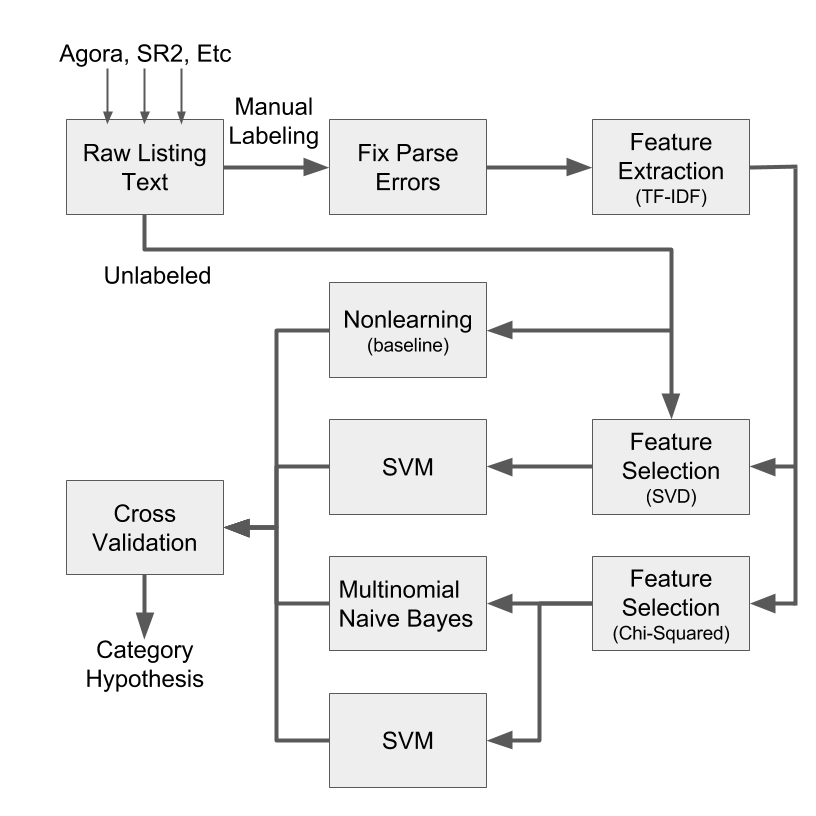
\includegraphics[width=0.85\linewidth]{pipeline}
        \caption{Data Pipeline}
    \end{center}
    \label{data_pipeline}
\end{figure}

We had $\frac{1}{3}$ of our data at the beginning of our algorithm design
process and had not used it for training or cross validation. We used our
processing pipeline to compute category predictions for each point the in test
set.

\subsection{Results}

The most important metric for our classification algorithm is categorization
accuracy. The accuracy for a test set is the proportion of labels that were
correctly assigned. For comparison, we compared the accuracy of our method with
three other algorithms.
\begin{itemize}
    \item A baseline model that used simple substring search, with substrings chosen by an online market expert.
					For example, if a product listing contained the text "xanax", then the listing was classified under "benzos".
    \item The $\chi^2$ test provides a simple way to remove features that are not correlated with any
					labeling, and is much faster than SVD.  However, it is also much less accurate and has a much higher output dimension than SVD.
    \item Multinomial Naive Bayes, using the same $\chi^2$ features.
\end{itemize}
The accuracy for each model is shown in Figure \ref{accuracy}. The figure shows
that our model outperformed several more simple models.

\begin{figure}[htbp]
    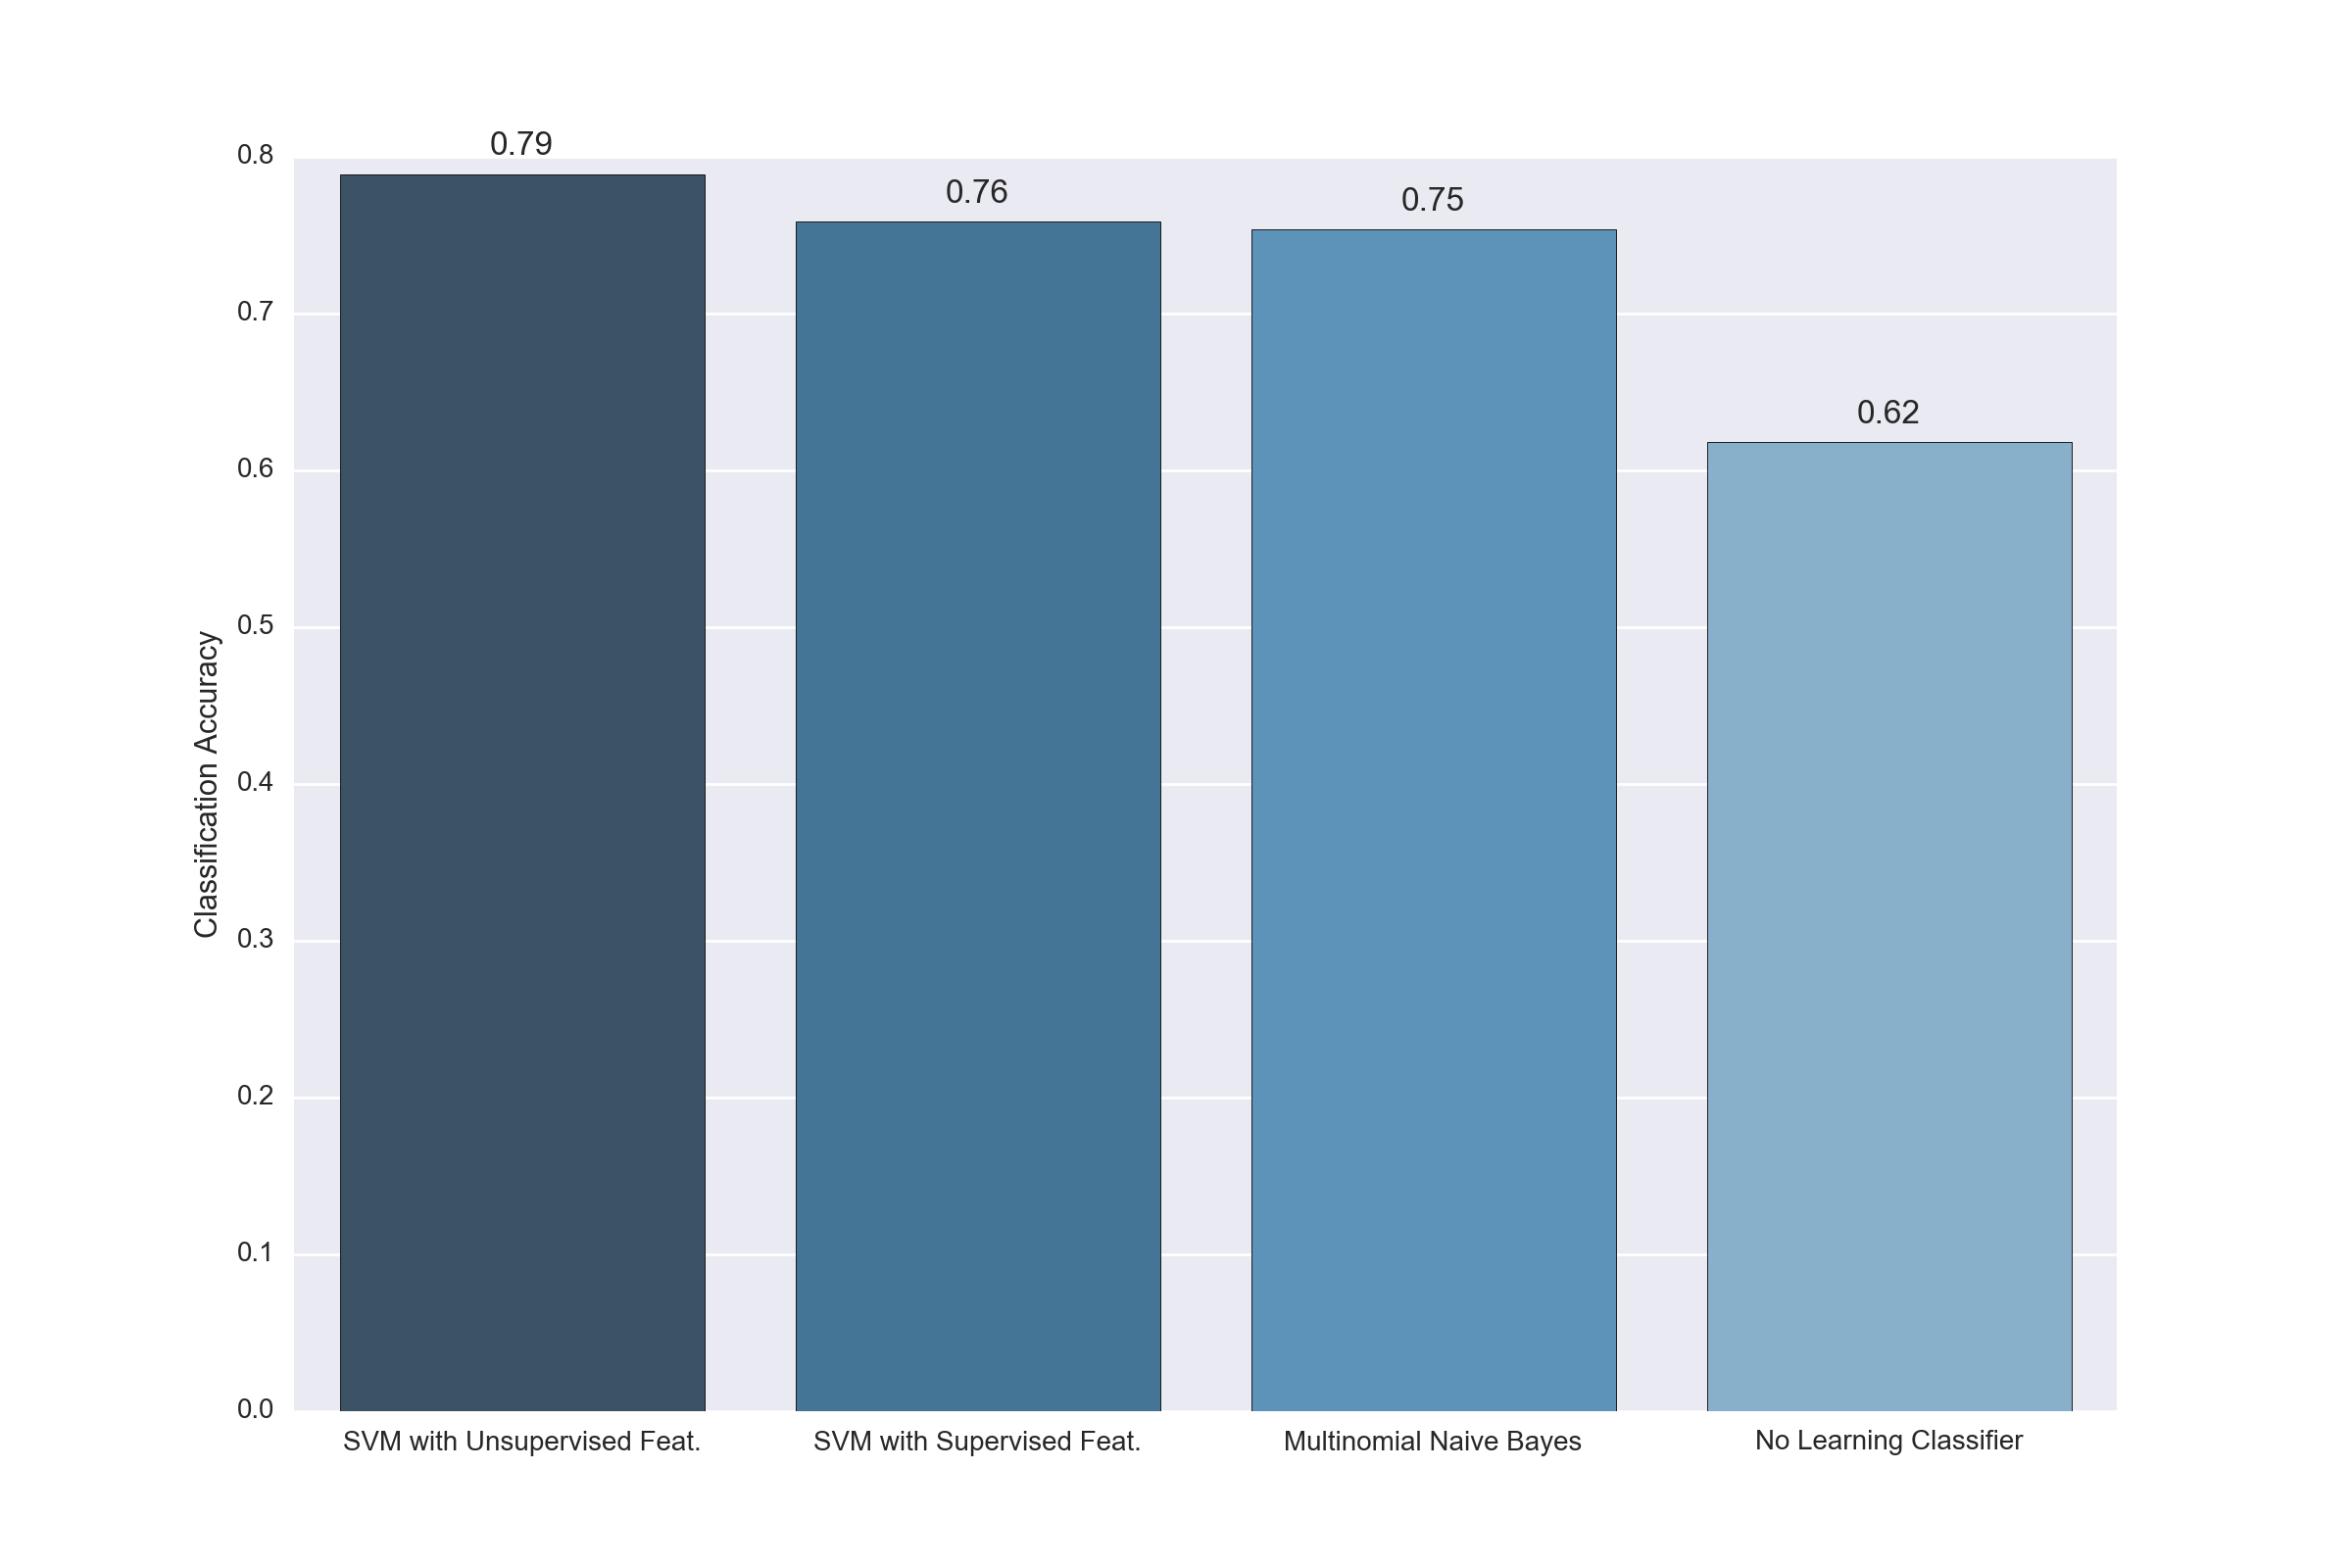
\includegraphics[width=\linewidth]{plots/models_accuracy}
    \caption{Comparison of Model Accuracies}
    \label{accuracy}
\end{figure}

\begin{table}[!ht]
    \begin{center}
        \begin{tabular}{| l | p{0.6\linewidth} |}
        \hline
        benzo & bensedin mot unmarked som bars 2mg diazepam xanax clonazepam zepose \\
        \hline
        dissociative &  purity reputation mxe 1000g methoxetamine chopping lab requested \\
        \hline
        ecstasy & 240 pressed pills mephedrone dutch red ecstasy express crystals 84 \\
        \hline
        misc & camel zolpidem lunesta eszopiclone caffeine phenargan zolab tranax  \\
        \hline
        opiate & 4mg 30mg heroine methadone opium codeine fentanyl naloxone tramadol \\
        \hline
        steroid & 10ml boldoject dianabol ml propionate sibutramine sibutramin test testosterone \\
        \hline
        psychedelic & buddha stand sheet babies mushrooms psilocybe hearts blotter nbome lsd \\
        \hline
        research chemical & fluoroamphetamine 36794 al 14g lad chiral dichloropane mdai fa apdb \\
        \hline
        prescription & mobic pseudoephedrine tadalafil generic dexamphetamine medications \\
        \hline
        stimulant & coke amphetamine check modafinil modalert adderall methamphetamine \\
        \hline
        marijuana & open grown dream crash kush weed hash wax taste sativa \\
        \hline
        other & size windows custom ways facebook account kinesiology book dpz guide \\
        \hline
        \end{tabular}
    \end{center}
    \caption{Top Tokens For Each Category}
    \label{category_tokens_table}
\end{table}



The precision recall curve compares shows the trade-off between precision (the
number of true positives over the total number of positives) vs recall (the
number of true positives over the number of true positives plus the false
negatives) as we vary our algorithm's parameters.
Figure \ref{prc_all} shows the precision-recall curve for our model.
\begin{figure}[htbp]
    \includegraphics[width=\linewidth]{plots/prc_all}
    \caption{Normalized Confusion Matrix}
    \label{prc_all}
\end{figure}

%%%%%%%%%%%%%%%%%%%%%%%%%%%%%%%%%%%%%%%%%%%%%%%%%%%%%%%%%%%%%%%%%%%%%%%%%%%%%%%%
% Confusion Matrix and discussion
\begin{figure}[htbp]
    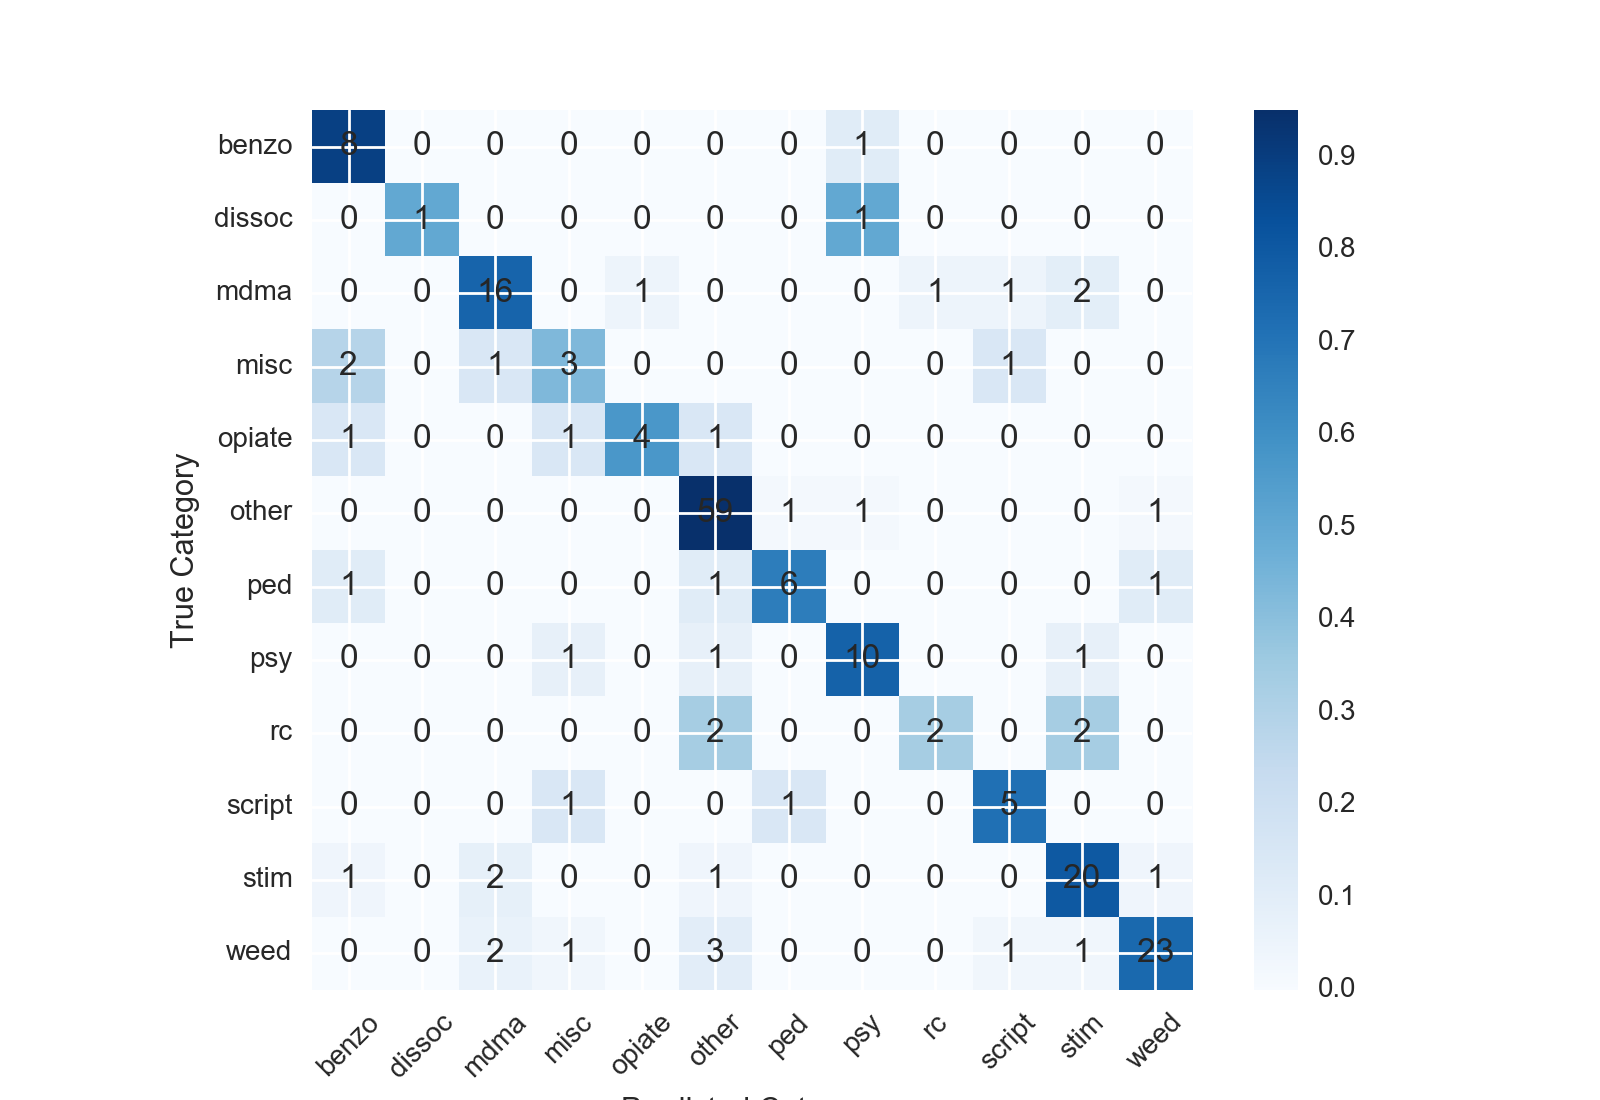
\includegraphics[width=\linewidth]{plots/confusion_matrix}
    \caption{Normalized Confusion Matrix}
    \label{confusion_matrix}
\end{figure}

Classification quality was not equal between each category. Figure \ref{confusion_matrix} shows the
confusion matrix of our algorithm on our test set. The grid position in row $i$ and column $j$ shows
the number of times a listing which is truly in category $i$ was classified by our algorithm as
category $j$. The values in the grid cells show the absolute number of test points, while the colors
show that number normalized by the true number of test points in each category.

The confusion matrix shows that our classifier was particularly bad at classifying the "other"
category.
We believe this is because of the large variety of "other" products available and the somewhat
arbitrary definition of the category. 
For example, we one category of goods we included in "other" was illegal digital goods, like movie downloads.
Because of this, drugs that had similar descriptions to unrelated products got misclassified as
"other".
To highlight this effect, our algorithm misclassified a strain of weed called "The Big Lebowski" as "other" because we had included a label for the movie download of "The Big Lebowski". See Table \ref{misclassified} for the complete example.

\begin{table}[!ht]
    \begin{center}
        \begin{tabular}{| l | p{0.6\linewidth} |}
        \hline
        True Category & Marijuana \\
        \hline
        Predicted Category & Other \\
        \hline
        Title & 1 4 Ounce The Big Lebowski \\
        \hline
        Description & The Big Lebowksi 2 3 week cure Indica sativa blend. Over the years pot has gotten a lot stronger especially with the advent of indoor hydroponic growing under metal halide and high pressure s...\\
        \hline
        \end{tabular}
    \end{center}
    \caption{Text of Typical Misprediction}
    \label{misclassified}
\end{table}


%%%%%%%%%%%%%%%%%%%%%%%%%%%%%%%%%%%%%%%%%%%%%%%%%%%%%%%%%%%%%%%%%%%%%%%%%%%%%%%%

% Did you do cross-validation, if so, how many folds? Before you list your results, make sure to
% list and explain what your primary metrics are: accuracy, precision, AUC, etc. Provide equations
% for the metrics if necessary. For results, you want to have a mixture of tables and plots. If you
% are solving a classification problem, you should include a confusion matrix or AUC/AUPRC curves.
% Include performance metrics such as precision, recall, and accuracy. You should have both
% quantitative and qualitative results. To reiterate, you must have both quantitative and
% qualitative results! This includes unsupervised learning (talk with your project TA on how to
% quantify unsupervised methods). Include visualizations of results, heatmaps, examples of where
% your algorithm failed and a discussion of why certain algorithms failed or succeeded. In addition,
% explain whether you think you have overfit to your training set and what, if anything, you did to
% mitigate that. Make sure to discuss the figures/tables in your main text throughout this section.
% Your plots should include legends, axis labels, and have font sizes that are readable when
% printed.


\section{Future Work}
% For future work, if you had more time, more team members, or more computational resources, what would you explore?
In this project, our training and testing used data from only a single market.
The algorithm could be made more robust by including data from more sources.
Test data drawn from a broader source would also provide a better generalization estimate.

Additionally, our algorithm could have considered features other than the product listing text when classifing products. 
For example, we could have used product price as a feature.
However, as the amount of product is not listed in a consistant format, normalizing the prices would require extracting the amount of product being sold.


\section{Conclusion}
% Summarize your report and reiterate key points.
In this project, we developed a machine learning algorithm that can classify product listings according to the type of product being sold.
Our algorithm consisted of a pipeline using TF-IDF for feature extraction, SVD for feature selection, and SVM for final classification.
We then used cross-validation to select hyperparameters and tune our algorithm.

% Which algorithms were the highest-performing? 
We also evaluated our algorithm in comparison to several other models:
\begin{itemize}
    \item{A baseline model that used simple string search}
    \item{SVM with a Chi-Squared test for feature selection}
    \item{Multinomial Naive Bayes}
\end{itemize}

Our algorithm had an accuracy of 77\% compared to the baseline accuracy of 62\%.
Our algorithm also outperformed the alternate SVM and multinomial models.

% Why do you think that some algorithms worked better than others?
Our algorithm was able to outperform the alternate models because it was able to take advantage of structure in the large unlabeled dataset.
In this project, we had a small amount of labeled data, and a very large amount of unlabeled data.
The SVD we use is performed on the unlabeled data, which helps to expose structure not captured by the labeled data.
We then project our labeled data onto the vector space chosen by the SVD and train our SVM on the result.
This allows to take advantage of both our unlabeled and labeled data in selecting our decision boundry.

\begin{figure}[htbp]
    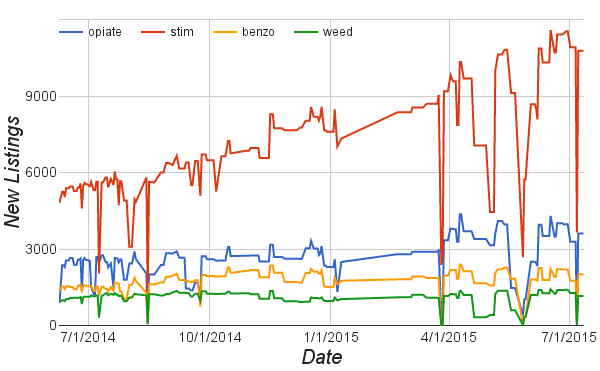
\includegraphics[width=\linewidth]{plots/new_categories_graph}
    \caption{New Listings By Category On Agora}
\end{figure}

We also used our classifier to measure the number of new products by category over time.
We found that by far the most common product listed on Agora is stimulants.
Interestingly, this was significantly different than an earlier anonymous market, The Silk Road,
where marijuana was the most common listed product, with stimulants a distant fourth\cite{christin-silkroad}.

This also matches reports from user and vendor forums, many of whom have complained that the
legalization of marijuana has reduced the profitability of selling online.
Conversely, amphetamine demand has dramatically risen, while production costs have dropped.
This has resulted in an apparent increase in product listings.
As far as we are aware, we are the first to rigorously document this switch.
This shows that our algorithm is extremely useful in practice, particularly for law enforcement and researchers.



% Put references on a page by themselves when using endfloat and the
% captionsoff option.
\newpage


% trigger a \newpage just before the given reference
% number - used to balance the columns on the last page
% adjust value as needed - may need to be readjusted if
% the document is modified later
%\IEEEtriggeratref{8}
% The "triggered" command can be changed if desired:
%\IEEEtriggercmd{\enlargethispage{-5in}}
\nocite{*}

% references section
\bibliographystyle{IEEEtran}
\bibliography{IEEEabrv,bibliography}

% You can push biographies down or up by placing
% a \vfill before or after them. The appropriate
% use of \vfill depends on what kind of text is
% on the last page and whether or not the columns
% are being equalized.

%\vfill

% Can be used to pull up biographies so that the bottom of the last one
% is flush with the other column.
%\enlargethispage{-5in}


\end{document}
